%===============================================================================
\begin{frame}[t]
    \frametitle{Структурная схема проекта}
    \begin{block}{} %{\centering Архитектура проекта}
        \vspace{1mm}
        \centering 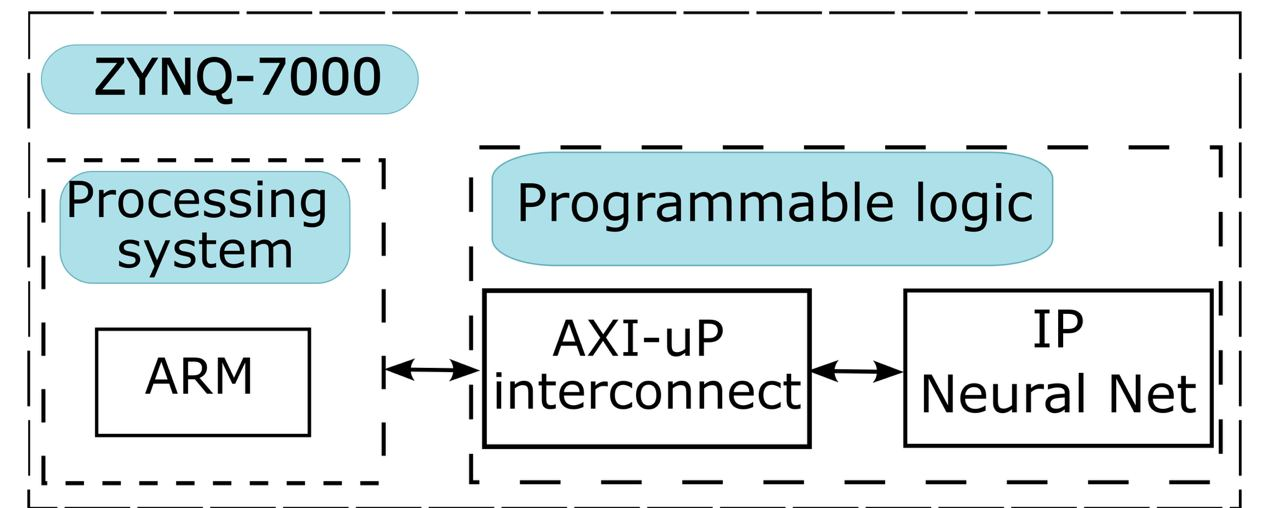
\includegraphics[width = 0.7\textwidth]{pics/str.jpg}
        % \includesvg[height = 0.4\textheight]{basic_AE.svg}    
        \begin{itemize}\small
            \item Подключение PL блока к PS осуществляется с помощью AXI4-Lite и uP интерфейсов.
        \end{itemize}     
    \end{block}  
\end{frame}
%===============================================================================
\begin{frame}[t]
    \frametitle{Эксперимент}
    \begin{columns}[T]
        \column{0.4\textwidth}
    
        \begin{itemize}
            \item Используется набор данных MNIST (10 тыс. изображений рукописных цифр $28 \times 28$)
            \item Данные подаются последовательно из процессорной системы
            \item Результаты группируются в виде матрицы спутывания
            \item Полученная точность составляет 96,6\%
        \end{itemize}
    
        \column{0.6\textwidth}
        \begin{block}{\centering}
            \vspace{1mm}
            \centering
            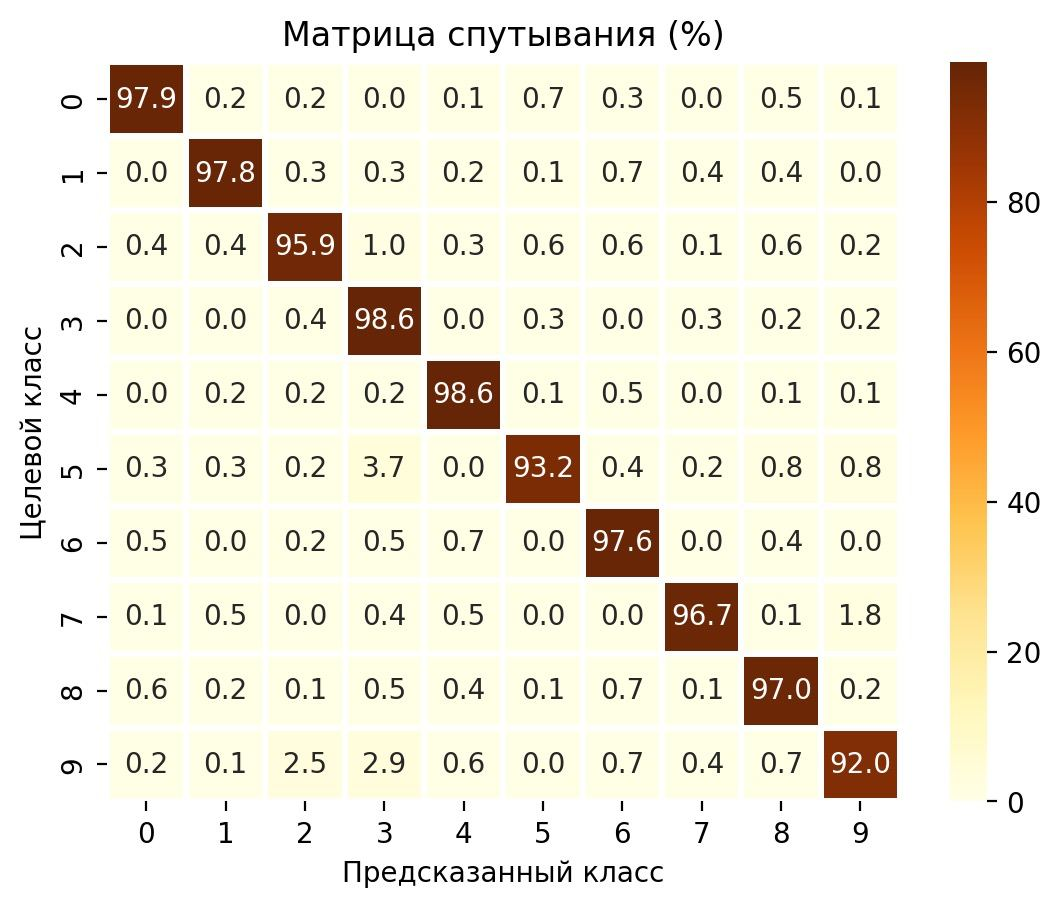
\includegraphics[width = 0.8\textwidth]{pics/m.jpg} 
            % \includesvg[height = 0.5\textheight]{RGB_multidim_data.svg}        
        \end{block}
    \end{columns}

\end{frame}
%===============================================================================